\chapter{StarCraft}
\label{ch:starcraft}
\emph{StarCraft} is a \emph{real-time strategy} (RTS) game released by Blizzard Entertainment in 1998. Controlling structures and troops, players seek to expand their economy, technology and army until they can eliminate all opponents. Players take the role as one of three different races: \emph{Terran}, \emph{Zerg} or \emph{Protoss}. These determine which buildings and troops are available to the players, and while mechanically similar they are very different strategically. The expansion \emph{StarCraft: Brood War}, also released in 1998, increased the rooster of troops available among other things.

\begin{figure}
	\centering
	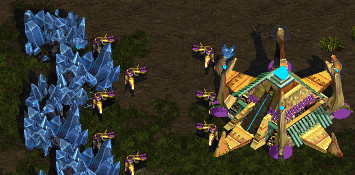
\includegraphics{figures/Base}
	\caption{A screenshot of units. Mineral resources to the left, workers in the middle and a depot structure to the right.}
	\label{fig:base}
\end{figure}

Players interact with game through \emph{units} which take the form of troops and buildings (see figure \ref{fig:base}). These can be given \emph{commands} by players, such as move, attack or build. Buildings can be commanded as well, capable of producing additional non-building units or upgrade to new technologies. Resources must be acquired to build structures, train troops or upgrade technologies. Resources are placed around on the map, and must be gathered by worker units, the only units capable of doing so.

The map is covered in the \emph{fog-of-war} which limits players' visibility to only their own units and their surroundings. Everything within the fog-of-war is hidden, including opponents' units within.

In multi-player matches, each player starts with a single structure and a few worker units. Each unit is identified with a player color, controllable by only that player. The goals is then to destroy all the opponents' structures, which is done by amassing an army and attacking. Each match is played on one of many \emph{maps}, which determines the terrain, resource and start locations. These factors have great impact on the pacing and player strategies. With a large amount of different unit- and building types available, the players compete by using the right types to counter their opponents' units. Players must adapt to the battlefield situation, as there is always a counter-strategy to every strategy.